% ЕМТ 2025, XI клас — точен LaTeX препис от официалните файлове в Klasirane.com.
% Условия: https://klasirane.com/api/competitions/EMT/All/2025/11%20%D0%BA%D0%BB/probs
% SHA-256 (условия): 8cd18f0d44ff8accd50fbb879ae6e08e025fc3ef9f73d5cddac4692d430ae23c
% Решения: https://klasirane.com/api/competitions/EMT/All/2025/11%20%D0%BA%D0%BB/sol
% SHA-256 (решения): 7b21ca22255e9b0546e872c30876f983398188dfb0cf6c57b901769a56c117c8
% Точковите оценки, правописът, формулировките и видимите печатни грешки са запазени от източника.
% Файлът с условията е едностранично сканирано изображение; видимата страница е проверена пряко.

Задача 11.1. Даден е остроъгълен триъгълник $ABC$ с ортоцентър $H$. Върху страната $BC$ е избрана произволна точка $D$. Нека перпендикулярът от $D$ към $BC$ пресича $BH$ и $CH$ в съответно точките $X$ и $Y$. Ако $H_1$ е ортоцентърът на триъгълника $HXY$, да се докаже, че $A$, $H_1$ и $D$ лежат на една права.

Решение. (Първи начин) Нека без загуба на общност да допуснем, че $D$ лежи на отсечката $PC$, където $P$ е петата на височината от $A$ към $BC$. И нека правата $HH_1$ пресича правата $AC$ в точка $Q$. От $YH_1\perp BH$ и $CQ\perp BH$ следва, че $H_1Y\parallel CQ$.

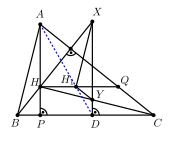
\includegraphics[max width=0.48\textwidth, alt={Официалната фигура към решение 11.1 с триъгълника ABC и точките D, H, H1, P, Q, X и Y}, center]{assets/11-1-geometry.svg}

Сега от Талес имаме, че $\frac{HH_1}{HQ}=\frac{HY}{HC}$. От друга страна $HP\parallel YD$, защото и двете са перпендикулярни на $BC$. Oтново от Талес получаваме, че $\frac{HY}{HC}=\frac{PD}{PC}$. Следователно $\frac{HH_1}{HQ}=\frac{PD}{PC}=\frac{HY}{HC}$. Като добавим и факта, че $HQ\parallel PC$, защото и двете са перпендикулярни на $AH$, получаваме, че $A$, $H_1$ и $D$ лежат на една права.

(Втори начин) Нека без ограничение $D$ и $B$ лежат в различни полуравнини спрямо $AH$ и $AH\cap BC=P$, $HH_1\cap XY=R$. Понеже $AH\parallel DR$, от теоремата на Талес исканото е еквивалентно на $\frac{AH}{HH_1}=\frac{RD}{RH_1}$. Тъй като $HPDR$ е правоъгълник, то $DR=HP$ и свеждаме до доказването на $\frac{AH}{HP}=\frac{HH_1}{RH_1}$. Обаче $\angle HYX=\angle DPC=90^\circ-\angle DCP=\angle ABC$ и аналогично $\angle HXY=\angle ACB$, следователно $\triangle ABC\sim\triangle HXY$ и желаното равенство представлява съответни елементи в тези триъгълници.

Оценяване. (6 точки) 2 т. за забелязване, че $H_1$ е пресечна точка на правата $AD$ и правата през $H$ успоредна на $BC$; 4 т. за довършване.

Задача 11.2. Дадена е аритметична прогресия от положителни числа $a_1$, $a_2$, $\ldots$, $a_n$, за която са изпълнени условията:

$$\frac{1}{a_1\cdot a_2}+\frac{1}{a_2\cdot a_3}+\cdots+\frac{1}{a_{n-1}\cdot a_n}=\frac12,$$

$$\frac{1}{\sqrt{a_1}+\sqrt{a_2}}+\frac{1}{\sqrt{a_2}+\sqrt{a_3}}+\cdots+\frac{1}{\sqrt{a_{n-1}}+\sqrt{a_n}}=9.$$

Дадено е, че $a_1$ е корен на уравнението

$$2x^2-13x+36=\sqrt{x}(11x-36).$$

Намерете броя на числата в аритметичната прогресия.

Отговор: $n=73$

Решение. По метода на Хорнер разлагаме

$$2x^2-11x\sqrt{x}-13x+36\sqrt{x}+36=(\sqrt{x}-2)(\sqrt{x}-6)(\sqrt{x}+1)(2\sqrt{x}+3)=0.$$

Поради факта, че $\sqrt{x}$ е неотрицателно, решенията на това уравнение са $x=36$ и $x=4$, тоест имаме двата случая $a_1=36$ и $a_1=4$.

Нека разликата на аритметичната прогресия да е $d$. Непосредствено се вижда, че при $d=0$ няма константна аритметична прогресия удовлетворяваща дадените условия. Нататък считаме, че $d\ne0$. От

$$\frac1d\left(\frac1{a_i}-\frac1{a_{i+1}}\right)=\frac1d\cdot\frac{a_{i+1}-a_i}{a_i\cdot a_{i+1}}=\frac1{a_i\cdot a_{i+1}},$$

следва

$$\begin{aligned}
\frac{1}{a_1\cdot a_2}+\frac{1}{a_2\cdot a_3}+\cdots+\frac{1}{a_{n-1}\cdot a_n}
&=\frac1d\left(\frac1{a_1}-\frac1{a_2}+\frac1{a_2}-\frac1{a_3}+\cdots+\frac1{a_{n-1}}-\frac1{a_n}\right)\\
&=\frac1d\frac{a_n-a_1}{a_1\cdot a_n}=\frac{n-1}{a_1\cdot a_n}.
\end{aligned}$$

Освен това, да забележим, че

$$\frac1{\sqrt{a_k}+\sqrt{a_{k+1}}}=\frac{\sqrt{a_{k+1}}-\sqrt{a_k}}{\sqrt{a_{k+1}}-\sqrt{a_k}}\cdot\frac1{\sqrt{a_k}+\sqrt{a_{k+1}}}=\frac{\sqrt{a_{k+1}}-\sqrt{a_k}}{a_{k+1}-a_k}=\frac{\sqrt{a_{k+1}}-\sqrt{a_k}}d,$$

от което получаваме

$$\begin{aligned}
\frac1{\sqrt{a_1}+\sqrt{a_2}}+\frac1{\sqrt{a_2}+\sqrt{a_3}}+\cdots+\frac1{\sqrt{a_{n-1}}+\sqrt{a_n}}
&=\frac{\sqrt{a_2}-\sqrt{a_1}}d+\frac{\sqrt{a_3}-\sqrt{a_2}}d+\cdots+\frac{\sqrt{a_n}-\sqrt{a_{n-1}}}d\\
&=\frac{\sqrt{a_n}-\sqrt{a_1}}d\cdot\frac{\sqrt{a_1}+\sqrt{a_n}}{\sqrt{a_1}+\sqrt{a_n}}\\
&=\frac{a_n-a_1}{d(\sqrt{a_1}+\sqrt{a_n})}=\frac{n-1}{\sqrt{a_1}+\sqrt{a_n}}.
\end{aligned}$$

Значи имаме: $\frac{n-1}{\sqrt{a_1}+\sqrt{a_n}}=9$ и $\frac{n-1}{a_1\cdot a_n}=\frac12$. Като разделим тези равенства и положим $a_n=t^2$ ($t\ge0$) ще получим, че

$$\begin{aligned}
a_1\cdot a_n&=18\cdot(\sqrt{a_1}+\sqrt{a_n})\\
a_1\cdot t^2&=18t+18\sqrt{a_1}\\
a_1\cdot t^2-18t-18\sqrt{a_1}&=0\\
t&=\frac{18\pm\sqrt{18^2+4a_1\cdot18\sqrt{a_1}}}{2a_1}.
\end{aligned}$$

Решаваме уравнението за двете възможни стойности: $a_1=4$ и $a_1=36$ и получаваме съответно $t=6$, $t=-\frac32$ и $t=2$, $t=-\frac32$. Тъй като $t\ge0$, единствено възможно е $a_n=36$ и $a_n=4$. В двата случая получаваме еднакви краища на аритметичната прогресия. Освен това знаем, че $\frac{n-1}{a_1a_2}=\frac{n-1}{4\cdot36}=\frac{n-1}{144}=\frac12$, следователно и в двата случая аритметичната прогресия има 73 члена, а разликата ѝ е $\frac49$ при $a_1=4$ и $-\frac49$ при $a_1=36$.

Оценяване. (6 точки) 2 т. за намиране $a_1=4$ или $a_1=36$; 1 т. за намиране на сумата $\sum\frac1{a_i\cdot a_{i+1}}$; 1 т. за намиране на сумата $\sum\frac1{\sqrt{a_i}+\sqrt{a_{i+1}}}$; 2 т. за отговор и довършване.

Задача 11.3. С $P_n$, $n\ge3$ означаваме правилен $n$-ъгълник, всеки два върха на който са свързани с отсечка. Едно естествено число $k\ge2$ ще наричаме лабилно, ако за някое $n\ge3$, съществува оцветяване на отсечките в $P_n$ в точно $k$ цвята, така че за всяко подмножество $X$ от върхове на $P_n$, точният брой на цветовете, в които са оцветени отсечките, свързващи двойките върхове от $X$, не е равен на $k-1$. Да се намерят всички лабилни числа $k$.

Отговор: $k\in\{i\in\mathbb N:i\ge2\}\setminus\{2,4\}$.

Решение. Ще покажем, че всички лабилни числа са $k\ge2$, $k\ne2,4$. Числото $k=2$ не е лабилно, защото за всяко оцветяване на $P_n$ в два цвята избираме множество $X$ от точно две точки. Отсечката между тях е е оцветена в точно един цвят. Числото $k=3$ е лабилно. Наистина, ако вземем $P_3$, няма подмножество на върховете му, определящи отсечки оцветени в точно 2 цвята.

Числото $k=4$ не е лабилно. Ще докажем, че ако отсечките на $P_n$ са оцветени в 4 цвята, винаги може да намерим подмножество $X$ на върховете, определящо отсечки оцветени в точно 3 цвята. Да вземем $P_n$, отсечките на което са оцветени в точно 4 цвята. Нека $X'$ е подмножество на върховете в $P_n$ с минимален брой елементи, такова че отсечките с краища в $X'$ да са оцветени в точно 4 цвята. Очевидно $|X'|\ge4$. Нека $v\in X'$ е произволен връх в $X'$. Съгласно екстремалността на $X'$, ако премахнем $v$ и всички отсечки с край във $v$, ще получим множеството $X'\setminus\{v\}$, което има по-малко на брой върхове от $X'$ и значи броят на цветовете $m$, които се срещат измежду отсечките с краища в $X'\setminus\{v\}$ е най-много 3. Ако $m=3$ сме готови. Да допуснем, че $m\le2$. Тогава, има два различни цвята, които се срещат в отсечките, които свързват $v$ с върховете в $X'\setminus\{v\}$, но нито един от тях не се среща в оцветяването на отсечките с върхове в $X'\setminus\{v\}$. Нека отсечките $vz$ и $vw$, $z,w\in C\setminus\{v\}$ са оцветени в тези два цвята. Тъй като отсечката $zw$ не може да е е оцветена в някой от горните два цвята, то множеството $X=\{v,w,z\}$ определя три отсечки в три различни цвята. Окончателно, $k=4$ не е лабилно.

Ще покажем, че всяко $k\ge5$ е лабилно. Да номерираме цветовете от 1 до $k$ и вземем $P_{k-1}$. Оцветяваме $v_iv_{i+1}$ в цвят $i$, за $i=1,2,\ldots,k-1$ (приемаме, че $v_k\equiv v_1$). Всички останали отсечки оцветяваме в цвят $k$. Да допуснем, че съществува множество $X$, което да генерира $k-1$ оцветяване на отсечките в него. Тъй като $X$ има по-малко върхове от $P_n$, то съществува $v_i$ такова, че $v_i\notin X$. Но тогава, нито цвят $i$ нито цвят $i-1$ (за $i=1$, втория цвят е $k-1$) се срещат в оцветените отсечки с краища в $X$. Противоречие. Следователно числата $k\ge5$ са лабилни.

Оценяване. (7 точки) по 1 т. за случаите $k=2,3$; 3 т. за случая $k=4$; 2 т. за случая $k\ge5$.

Задача 11.4. Дадена е редицата от естествени числа $(a_n)_{n=1}^{\infty}$, като за всяко $m\in\mathbb N$ са изпълнени условията:

• ако $a_i\equiv a_j\pmod m$ за някои $i,j\in\mathbb N$, то $a_{i+1}\equiv a_{j+1}\pmod m$

• ако $a_i\equiv0\pmod m$ за някое $i\in\mathbb N$, то $a_{i+1}\equiv0\pmod m$.

Докажете, че за всеки $a\in\mathbb N$, $b\in\mathbb Z$ съществува $n\in\mathbb N$ такова, че

$$n+a_n\equiv b\pmod a.$$

Решение. Ще проведем индукция по $a$. Ще докажем, че за всяко $N\in\mathbb N$, съществува $n\ge N$, което удовлетворява (1). За $a=1$ твърдението е тривиално. Нека $a\in\mathbb N$, $a\ge2$ и нека сме доказали твърдението за всички по-малки стойности от $a$. Да предположим първо, че редицата има член с остатък 0 по модул $a$. Тогава $a_n\equiv0\pmod a$ за всички достатъчно големи $n$ и е достатъчно да вземем такова $n$, за което $n\equiv b\pmod a$.

Нека сега $a_n\not\equiv0\pmod a$, $\forall n\in\mathbb N$. Тогава тя е периодична по модул $a$ с период $k$ от някое място нататък. Т.е. $a_{i+kj}\equiv a_i\pmod a$ за всяко $j\in\mathbb N$ и всяко $i\ge N$, където $N\in\mathbb N$. Нека $k$ e най-малкия такъв период. Това означава, че числата $a_i,a_{i+1},\ldots,a_{i+k-1}$ дават различни ненулеви остатъци по модул $a$ и значи $k<a$. И така

$$(i+kj)+a_{i+kj}-b=a_i+i-b+kj\pmod a.$$

Нека $d=(k,a)$ и $k=k_1d$, $a=a_1d$. Да забележим, че за всяко $j_1\in\mathbb N$ съществува $j\in\mathbb N$ такова, че $jk+j_1d\equiv0\pmod a$. Наистина, $jk+j_1d=(jk_1+j_1)d$. От друга страна, тъй като $(k_1,a_1)=1$, можем да намерим $j\in\mathbb N$ така, че $a_1\mid jk_1+j_1$, което означава $a\mid jk+j_1d$.

И така, за да докажем, че съществуват $i,j\in\mathbb N$, $i\ge N$, които удовлетворяват:

$$(a_i+i-b)+kj\equiv0\pmod a$$

е достатъчно да намерим $i\ge N$, такова че $d\mid a_i+i-b$. Но от $k<a$ следва $d<a$. И така, сведохме задачата до намиране на $i\ge N$, за което

$$a_i+i\equiv b\pmod d.$$

Това може да се направи съгласно индукционното предположение.

Оценяване. (7 точки) 2 т. за доказване, че ако $(k,a)=1$, където $k$ е периода на редицата по mod $a$, то всички остатъци (mod $k$) са възможни; 5 т. за доказване на общия случай.
